%
% revised in Jan, 18th, 2008
% problems left behind:
% 1   whether we can have such extension:
% \begin{equation}\label{GROUPeq:8}
%     \hat{O}_{R}[\Psi\Phi] = (\hat{O}_{R}\Psi)(\hat{O}_{R}\Phi)
%     \end{equation}
%     I am not sure that whether it's correct.  2 vanishing integrals
%     is not fully finished, something is still missing; perhaps
%     better to rewrite some of the content
%
%
%

%%%%%%%%%%%%%%%%%%%%%%%%%%%%%%%%%%%%%%%%%%%%%
\chapter{Group Theory in Quantum Chemistry}
%
% introduction: what's the group theory origin.
%
%
Group theory is a branch of pure mathematics, but it plays an
important role in quantum mechanics. Qualitative information about
molecular wave function and its property can always be obtained from
the symmetry of molecule. In essence, the symmetry of molecule is one
of its fundamental property, which is originated from the uncertainty
principle of the quantum particles.

Before stepping in the detailed discussion, it's very interesting to
take a general view about the comparison between classic mechanics and
quantum mechanics. In the macroscopic world, there never has two
objects that are exactly same with each other; but in the quantum
world, because of the uncertainty principle, if the particles belongs
to the same type, for example, two electrons, and two hydrogen atoms;
it's impossible to distinguish them between each other. So two
electrons actually are the same, and so as the atoms.  Thus the
symmetry of the molecule is a result of the uncertainty principle. In
a sense, the symmetry is some kind of inherent and fundamental
property embedded in the molecule. The description here in this
chapter is basically taken from two books given by Bishop\cite{Bishop}
and Cotton\cite{Cotton}.

%%%%%%%%%%%%%%%%%%%%%%%%%%%%%%%%%%%%%%%%%%%%
\section{The concept of symmetry operation}\label{GROUP13}
% 1 definition of the symmetry operation and symmetry element as well
% as their difference 2 how to understand the symmetry operation
%
%
Before we started, it's necessary for us to distinguish an important
concept: that the difference between symmetry operation and symmetry
element. Symmetry operation is the transformation of a body such that
the final position is physically indistinguishable from the initial
position. Symmetry elements is the geometrical entity (point, line or
plane) with respect to which a symmetry operation is carried out. So
we can see that they are conceptually different.  Furthermore, the
point group we will discuss here, is related to the group of symmetry
operations; and the symmetry element is a way to help us to
intuitively understand the symmetry operation.

The introduction of the concept of symmetry operation is vital to the
use of group theory in the chemistry. This concept generalizes the
intrinsic symmetric property of the molecules, through this concept
the application of the group theory is made possible.  Therefore, the
symmetry operation is the most fundamental concept in this subject.

How can we understand the symmetry operations? To some extent, the
symmetry operation is similar to the operator in the quantum
mechanics. Symmetry operation is only some general and abstract form
of operation, as we use different ``bases'' on which the symmetry
operation is applied, there will be accordingly different ways to
represent the same symmetry operation. For example, if we use the
coordinates of an atom (the base is the coordinates), then the
symmetry operation will naturally correspond to some $3\times 3$
matrix which converts one position of atom to another. If we use the
coordinates from s specific molecule (for example, a molecule contains
$9$ atoms), then the same symmetry operation will be some $27\times
27$ matrix working on the coordinates of the bunch of atoms. On the
other hand, if the atom orbitals(or more specifically to say, the
basis functions) are used, the symmetry operation will be the matrix
that describing the mixture of the corresponding orbitals. However, no
matter what kind of representations the symmetry operation is chosen
to be, they all reflect the same essence behind it; that's why we can
use the abstract group theory to describe such generalized concept.

%%%%%%%%%%%%%%%%%%%%%%%%%%%%%%%%%%%%%%%%%

\subsection{Fundamental symmetry operations}
%
% 1 five fundamental symmetry operations 2 why the Sn is fundamental?
% 3 further discussion to the Sn
%

There are five fundamental symmetry operations; in a sense that all
the other symmetry operations can be composed from them.
\begin{itemize}
\item rotation over an axis ($C_{n}$)
\item inversion related to a point ( i )
\item reflection through a mirror of plane ($\sigma$)
\item rotation over an axis then plus reflection through a mirror of
  plane (here the index of h means that the plane is vertical to the
  axis) ($S_{n} = \sigma_{h} C_{n}$)
\item identical operation ($E$)
\end{itemize}

It's very natural to understand the symmetry operation of reflection,
inversion and rotation. Such operations are represented by the
fundamental symmetry elements of point, axis and plane.  Identical
operation of $E$ makes the molecule unchanged, actually it's the
identity element in the point group. Any group can not be short of the
identity element, so it's a fundamental operation.

Here is an interesting question that why the rotation-reflection
$S_{n}$ is a fundamental operation? Actually we can find that there
has some molecule that only has the $S_{n}$ operation, where the
rotation operation and reflection operation are absent. Therefore,
$S_{n}$ is symmetry operation independent of $C_{n}$ and
$\sigma_{h}$. Here below the (\ref{GROUP11}) shows that how to make a
$S_{n}$ symmetry operation.

\begin{figure}[htp]
  \begin{center}
    \includegraphics[scale=0.7]{s4.eps}
    \caption{an example that how to make S4 symmetry operation}
    \label{GROUP11}
  \end{center}
\end{figure}

To further understand this situation, there are several general rules
respect to the connection between $S_{n}$ and $C_{n}, \sigma$.
\begin{itemize}
\item if $n$ is odd number, the $S_{n}$ is the direct product of
  $C_{n}$ and $\sigma_{h}$; here the $S_{n}$ is the combination
  between the $C_{n}$ and $\sigma$. the case of $S_{3}$ clearly
  demonstrates such rules.
\item if $n$ is an even number, the case should be divided into two
  subgroups:
  \begin{itemize}
  \item if the $n=4k$, $S_{n}$ is an unique and independent symmetry
    operation, together with the $C_{\frac{n}{2}}$ symmetry operation.
  \item for the other cases, the $S_{n}$ is composed by the
    $C_{\frac{n}{2}}$ and $\sigma_{h}$. The case of $S_{6}$ will show
    this.
  \end{itemize}
\end{itemize}

the $S_{4}$ is:
\begin{eqnarray}\label{GROUPeq:2}
  S^{1}_{4} &=& \sigma_{h}C^{1}_{4}  \nonumber \\
  S^{2}_{4} &=& \sigma^{2}_{h}C^{2}_{4} = C^{1}_{2} \nonumber \\
  S^{3}_{4} &=& \sigma_{h}C^{3}_{4}   \nonumber \\
  S^{4}_{4} &=& E  \nonumber \\
  S^{i}_{4} &=& S^{i-4}_{4} (i > 4)
\end{eqnarray}

the $S_{3}$ is:
\begin{eqnarray}\label{GROUPeq:3}
  S^{1}_{3} &=& \sigma_{h}C^{1}_{3}                 \nonumber \\
  S^{2}_{3} &=& \sigma^{2}_{h}C^{2}_{3} = C^{2}_{3} \nonumber \\
  S^{3}_{3} &=& \sigma_{h}C^{3}_{3} = \sigma_{h}    \nonumber \\
  S^{4}_{3} &=& C^{1}_{3}                           \nonumber \\
  S^{5}_{3} &=& \sigma_{h}C^{2}_{3}                 \nonumber \\
  S^{6}_{3} &=& E
\end{eqnarray}
Here we can see that the $S_{3}$ reproduce the group of $C_{3}\otimes
\sigma_{h}$.


Now let's see the case of $S_{6}$.

\begin{eqnarray}\label{GROUPeq:4}
  S^{1}_{6} &=& \sigma_{h}C^{1}_{6}                 \nonumber \\
  S^{2}_{6} &=& \sigma^{2}_{h}C^{1}_{3} = C^{1}_{3} \nonumber \\
  S^{3}_{6} &=& \sigma_{h}C^{1}_{2} = i             \nonumber \\
  S^{4}_{6} &=& C^{2}_{3}                           \nonumber \\
  S^{5}_{6} &=& \sigma_{h}C^{5}_{6}                 \nonumber \\
  S^{6}_{6} &=& E
\end{eqnarray}

Hence, we can see that $S_{4k}$ is indecent of the $C_{n}$ and
$\sigma$, as in $S_{4}$ there's no $\sigma$ operation.

%%%%%%%%%%%%%%%%%%%%%%%%%%%%%%%%%%%%%%
\subsection{Algorithm between symmetry operation}
%
% 1 multiplication 2 commutative character 3 division 4 do not have
% addition ??
%
%
After setting up the fundamental symmetry operation, now in this
section we are going to demonstrate the algorithm between them.

The symmetry operations can be multiplied like operators. If $P$ and
$Q$ are two symmetry operations, their product of $PQ$ is naturally
the symmetry operation, too. Such multiplication is defined by the way
that first to apply the symmetry operation $Q$, then apply the
symmetry operation $P$:
\begin{equation}\label{}
  R = PQ
\end{equation}
Similar to the operator that the multiplication order is important.
Generally we have that $PQ \neq QP$. For example, for the $NH_{3}$
molecule it has $C_{3}$ and $\sigma$ operations, but we can see that
(this molecule has three reflection mirrors, they are labeled by $1$,
$2$ and $3$; separately):
\begin{equation}\label{}
  C_{3}^{1}\sigma_{1} = \sigma_{2} \quad  \sigma_{1}C_{3}^{1} =
  \sigma_{3}
\end{equation}
Therefore different order produce different results. However, there
exists some symmetry operations which do not care about the order:
$PQ=QP$, it's said that they are commutative. For example, $C_{3}$ and
$i$ are two commutative operations.

The multiplication between symmetry operations satisfy the commutation
rules below:
\begin{equation}\label{}
  (PQ)R = P(QR) = PQR
\end{equation}

The division algorithm, which is considered to be the counter
algorithm of the multiplication; can be defined that:
\begin{equation}\label{}
  PQ = E \Rightarrow P = Q^{-1}
\end{equation}
Since that any symmetry operation all has its counter operation (this
is the requirement by the group theory), thus for any point group, the
identity operation of $E$ always exists.

The algorithms concerned with the symmetry operation are mainly
related to the multiplication and division. It's interesting that
there's no addition, substraction etc. for the symmetry operations,
although in the quantum mechanics the operator has such operations.
That's because the addition etc. have no physical correspondence to
the symmetry operation, we do not know how to define the physical
process for the addition of two symmetry operations.

%%%%%%%%%%%%%%%%%%%%%%%%%%%%%%%%%%%%%%%%%%
\subsection{Product rules between symmetry operations}
%
% 1 we can form any groups based on the fundamental five symmetry
% operations 2 rules related to the product between symmetry
% operations 3 commutative rules between symmetry operations
%
So far, we have five fundamental symmetry operations, each of them can
form an independent group, and is labeled with an unique symmetry
element. They are:
\begin{itemize}
\item rotation group $C_{n}$: $\{E, C^{1}_{n}, C^{2}_{n}, \cdots,
  C^{n-1}_{n}\}$
\item reflection group $\sigma$: $\{E, \sigma \}$
\item inversion group $i$: $\{E, i \}$
\item rotation-reflection group $S_{n}$: $\{E, S^{1}_{n}, S^{2}_{n},
  \cdots, S^{n-1}_{n} \}$
\item identical group $E$: $\{E \}$
\end{itemize}

To some extent, the point group can be seen as the combination of such
five fundamental groups. Here between them, the presence of some
special symmetry elements will lead to the existence of some other
symmetry elements. In the content below, we are going to state such
summarized rules.
\begin{itemize}
\item combination of two rotation axes
  \begin{itemize}
  \item If two $C_{2}$ axes crosses with each other with an angle of
    $\frac{2\pi}{2n}$, there has a $C_{n}$ axis drilling through the
    cross point and perpendicular with the plane forming by the two
    $C_{2}$ axes. \\
    On the other hand, if there exists a $C_{n}$ axis and a $C_{2}$
    axis which is vertical to the $C_{n}$ axis; another $C_{2}$ axis
    which satisfies the above condition also holds its presence.
  \end{itemize}
\item combination of two mirrors
  \begin{itemize}
  \item If two mirrors crosses with each other with an angle of
    $\frac{2\pi}{2n}$, the cross line is a $C_{n}$ axis. On the other
    hand, if we have a $C_{n}$ axis and a reflection mirror through
    it, the rotation of the mirror leads to $n$ mirrors; with an angle
    of $\frac{2\pi}{2n}$ between any adjacent mirror pairs .
  \end{itemize}
\item combination between axis and mirror
  \begin{itemize}
  \item If we have an even $C_{n}$ axis with a mirror vertical to it,
    the cross point must be inversion point. Similarly if we have an
    inversion point and a mirror through it, we have a $C_{2}$ axis
    perpendicular to the mirror and through the inversion point.
  \end{itemize}
\end{itemize}

For the commutative character of the symmetry operation, it can be
proved that the pairs of symmetry operations below are always
commutative.
\begin{itemize}
\item two rotations around same axis
\item reflection through two perpendicular mirror
\item inversion and any rotation or reflection
\item rotations in succession on two vertical $C_{2}$ axis
\item rotation and reflection where the mirror vertical to the
  rotation axis
\end{itemize}


%%%%%%%%%%%%%%%%%%%%%%%%%%%%%%%%%%%%%
\section{Point group}
% 1 the definition of the point group, it's the unit for study 2 why
% called point group
%
What is the point group? The point group is the collection of all the
symmetry operations corresponding to some specifical molecules.
Mathematically, such collection forms an entire and complete group,
each possesses some individual characters. Here it's noted that the
point group is the unit for studying the application of group theory
on the chemistry.

The point group can always judged from the outside appearance of the
molecules. For example, the carbon dioxide molecule and the hydrogen
gas molecule are belonging to the same kind, because they own the same
kind of symmetry operations. On the other hand, the water molecule has
the different point group with the molecules mentioned above.

For a given molecule, since that the translation can not alter its
symmetry properties, all the symmetry operations should be all through
one point (this point is not varied for any symmetry operations. For a
single molecule, this point is its center of mass). Therefore the
point group is also called molecule group.


%%%%%%%%%%%%%%%%%%%%%%%%%%%%%%%%%%%%%%%%
\subsection{Conjugation in symmetry operations}
%
% 1 mathematically define the conjugation 2 three characters related
% to the conjugation 3 class definition, and it's not subgroup 4
% connection between commutation and conjugation
%
%
In a given point group of $G$, and if we have element of $C$ to make
operation $A$ and $B$ satisfy that $AC=CB$ (this is equivalent to
$C^{-1}AC = B$ since $C^{-1}$ always exists); then $A$ and $B$ are
called conjugated with each other.

We can prove the following characters related to the conjugation.
First, $A$ always conjugated to itself, that is we can always find
some $X$, to make $A = X^{-1}AX$.
\begin{equation}\label{}
  A^{-1}A = A^{-1}X^{-1}AX = (AX)^{-1}AX = E
\end{equation}
Here, we can always has $X = E$, but we may also find some others to
get the equation. For example, we have $i^{-1}C^{1}_{3}i = C^{1}_{3}$;
this is because $i$ and $C^{1}_{3}$ are commutative.

Second, $A$ conjugates with $B$ is equivalent to that $B$ conjugates
with $A$.
\begin{equation}\label{}
  X^{-1}AX = B \Leftrightarrow A = XBX^{-1}
\end{equation}

Third, if $A$ and $B$ are conjugated, and $B$ and $C$ are conjugated;
then $A$ and $C$ are conjugated, too.
\begin{align}\label{}
  P^{-1}AP = B  & \quad  Q^{-1}BQ = C \Rightarrow \nonumber \\
  Q^{-1}P^{-1}APQ &= R^{-1}AR = C
\end{align}
Here, $R = PQ$. Thus, the conjugated character can be passed from one
to another.

It's interesting to see that from the above three characters, it
implies that the operation of conjugation seems to be
``self-contained''. In fact, the elements which conjugated with each
other in a given group forms a ``class''; such class is some kind of
self-contained.

However, here the meaning of self-contained does not denote that the
class is forming a subgroup. For example, the symmetry operations for
the $NH_{3}$ molecule has been classified into three classes: $E$,
$\sigma_{1}, \sigma_{2},\sigma_{3}$ and $C^{1}_{3}, C^{2}_{3}$.  We
can see that in the second and third class there has not $E$ so that
they can not be subgroups.

On the other hand, there's no direct relations between commutation and
the conjugation. For example, the symmetry operations of $C^{i}_{n}
(i=1,2,\cdots,n)$ are commutative, but they are not in one class(from
the definition we can see this point. For any $C^{i}_{n} = P$ and
$C^{j}_{n} = Q$, and $i \neq j$; we always have $Q^{-1}PQ \equiv P$
for any $Q$). Generally, if the point group is an Abel kind, the
different elements in this group are in separate class, the number is
same to the order of the group.

%%%%%%%%%%%%%%%%%%%%%%%%%%%%%%%%%%%%%%%%
\subsection{Equivalent symmetry operations}
%
% this section talk about the conjugation in intuitional way
%
%
%
In the $C^{-}AC=B$, the $A$ and $B$ are called equivalent symmetry
operations. In this section, we are going to provide some way to
understand them in some intuitional way.

Firstly, we note that symmetry operation to the molecular coordinates
while retaining the coordinate system unchanged is identical to the
way that operation to the coordinate system while keeping the molecule
coordinates unchanged. This fact is easily understood in three
dimensional space. Therefore it turns out that we can interpret the
$C^{-}AC=B$ in this way:
\begin{quote}
  \begin{center}
    first the $C$ operation is made to the coordinate system to
    transform it to the new one, then in the new coordinate system the
    $A$ operation is made to the molecule coordinates; then finally
    the $C^{-}$ operation makes the new coordinates system restores to
    original one. From the equality, this process will generate the
    $B$ operation.
  \end{center}
\end{quote}

This is some very interesting interpretation. Here, it also implies
that why we call them as ``equivalent'' symmetry operations. Through
this process, we can clearly see that $A$ and $B$ are equivalent as
long as that they are the same symmetry operation by executing in
different coordinate system (here in the above interpretation, the $A$
happens in the new one changed by the $C$, and the $B$ happens in the
old one; but they lead to the same result).

On the other hand, by the similar way we can understand the equivalent
symmetry operation in another way; that if there exists a symmetry
operation working on the coordinate system, which is able to replace
$A$ by $B$ ($A$ and $B$ are also the symmetry operation in this
group); then $A$ and $B$ are conjugated with each other (they are also
the equivalent symmetry operations).

The understanding of this issue is same with the way above. Since that
we have $AC=CB$ for conjugated $A$ and $B$, if we can find the $C$
working on the coordinate system (that is equivalent to working on the
molecule itself); then the $AC$ means to change the coordinate system
by $C$, then apply the $A$ to the molecule. That is same to apply the
$B$ to the molecule, then change the coordinate system by $C$. Thus,
if $A$ and $B$ are conjugated; the effects of $B$ can be replaced by
the $A$, $A$ is doing in a new coordinate system. Such new system can
be transformed by one of the symmetry operation in this group.

Now let's take $C_{4v}$ as an example, it turns out that $C^{1}_{4}$
and $C^{3}_{4}$ are conjugated with each other. the $C^{1}_{4}$ makes
the molecule contrarotate for $\frac{2\pi}{4}$ angle, while the
$C^{3}_{4}$ makes the molecule rotate $\frac{2\pi}{4}$ in the
clockwise direction (the cartesian system used here are defined in the
figure of (\ref{GROUP12})).
\begin{figure}[htp]
  \begin{center}
    \includegraphics[scale=0.7]{coordinate_change.eps}
    \caption{coordinate changes by the $\sigma_{d}$} \label{GROUP12}
  \end{center}
\end{figure}

In the original coordinate system, the effects for both of $C^{1}_{4}$
and $C^{3}_{4}$ are:
\begin{eqnarray}
  % \nonumber to remove numbering (before each equation)
  C^{1}_{4}(z)[x,y] &\Rightarrow& [y,-x] \nonumber \\
  C^{3}_{4}(z)[x,y] &\Rightarrow& [-y,x]
\end{eqnarray}
Here it has a third symmetry operation of $\sigma_{d}$, which exchange
$x$ and $y$ ($\sigma_{d}[x,y] \Rightarrow [y,x]$).  Therefore, in the
new coordinate system indicating by the figure of (\ref{GROUP12}), we
have:
\begin{eqnarray}
  % \nonumber to remove numbering (before each equation)
  C^{1}_{4}(z)[x,y] \Leftrightarrow C^{1}_{4}(z)[y,x] (\text{old system})
  &\underrightarrow{\sigma_{d}}& [-y,x] \nonumber \\
  C^{3}_{4}(z)[x,y] \Leftrightarrow C^{3}_{4}(z)[y,x] (\text{old system})
  &\underrightarrow{\sigma_{d}}& [y,-x]
\end{eqnarray}
Thus, the $C^{1}_{4}$ and $C^{3}_{4}$ are equivalent symmetry
operations.

%%%%%%%%%%%%%%%%%%%%%%%%%%%%%%%%%%%%%%%%%%%%%%%%%%%%%%%%%%%%%%%%%%%%%%%%%%%%%%
\subsection{Class in point group}
%
% this section provide the details related to variety of the
% equivalent symmetry operation
%
So far we have fully understand the meaning of conjugation in the
point group. Now we can make some summarization that what kind of
symmetry operations are equivalent:

\begin{enumerate}
\item the identical operation and inversion operation.
  \begin{itemize}
  \item Since the both of $E$ and $i$ has only one element, $E$ and
    $i$ are individual class respectively.
  \end{itemize}
\item reflection
  \begin{itemize}
  \item If there's some operation to exchange their reflection mirror,
    such reflections related to these mirrors are in same class.
  \end{itemize}
\item $C_{n}$ and $S_{n}$ axis
  \begin{itemize}
  \item If there has mirrors containing the axis, or it has the
    $C_{2}$ vertical to the axis; the $C^{i}_{n}$ and $C^{n-i}_{n}$
    fall into same class, so as the $S^{i}_{n}$.
  \end{itemize}
\end{enumerate}

Finally we can make some extra example of $C_{4v}$ to classify the
principle with the $C_{n}$ and $S_{n}$ axis. The $C^{1}_{4}$ and
$C^{3}_{4}$ are conjugated for there is a mirror vertical to the
$C_{4}$ axis.

%%%%%%%%%%%%%%%%%%%%%%%%%%%%%%%%%%%%
\subsection{Classification of point group}
%
% this section provides the example of the point group
%
%
In the following content, we are going to give the systematical method
classification of the point group. From now on, for any molecules; we
can specify which point group it belongs to. All the symmetry
characters related to the molecule, is wholly demonstrated by the
details defined in its point group. We will begin from the simplest
case until reach to the complex ones.

$C_{1}$ group: \\
Actually this is only identical operation (E) related to this kind of
molecule, see figure of (\ref{GROUP1}).
\begin{figure}[htp]
  \begin{center}
    \includegraphics[scale=0.7]{molecule1.eps}
    \caption{C1 group} \label{GROUP1}
  \end{center}
\end{figure}

$C_{s}$ group: \\
$C_{s}$ is actually the group of $\sigma$; has two elements: $E$ and
$\sigma$, see figure of (\ref{GROUP2}).
\begin{figure}[htp]
  \begin{center}
    \includegraphics[scale=0.7]{molecule2.eps}
    \caption{CS group} \label{GROUP2}
  \end{center}
\end{figure}

$C_{n}$ group: \\
This group is identical to the group of $C_{n}$, only has a rotation
axis and identical operation, see figure of (\ref{GROUP3}).
\begin{figure}[htp]
  \begin{center}
    \includegraphics[scale=0.7]{molecule3.eps}
    \caption{C3 group} \label{GROUP3}
  \end{center}
\end{figure}

$C_{i}$ group: \\
This group is identical to the group of $i$, only has a inversion
operation and identical operation, see figure of (\ref{GROUP4}).
\begin{figure}[htp]
  \begin{center}
    \includegraphics[scale=0.7]{molecule4.eps}
    \caption{Ci group} \label{GROUP4}
  \end{center}
\end{figure}

$S_{n}$ group: \\
From the content above, we know that $S_{4}$ is some individual
group. Here below we present one example in the figure of
(\ref{GROUP7}).
\begin{figure}[htp]
  \begin{center}
    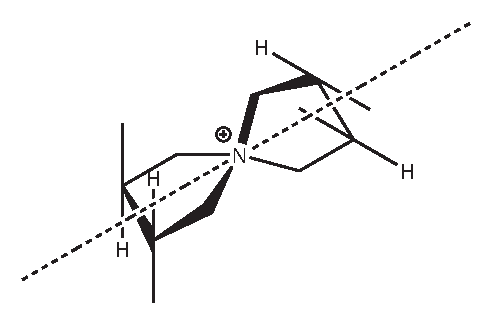
\includegraphics[scale=0.7]{S4_example.eps}
    \caption{S4 group} \label{GROUP7}
  \end{center}
\end{figure}

$C_{nv}$ group: \\
If we add a symmetry element of mirror to the $C_{n}$ axis, and this
mirror just contains the axis; from the analysis above we can know
that there must have n planes exist, as the rotation axis varies.
This group is called $C_{nv}$ group. The most famous example is
$H_{2}O$ molecule, see figure of (\ref{GROUP5}).
\begin{figure}[htp]
  \begin{center}
    \includegraphics[scale=0.7]{molecule5.eps}
    \caption{C2v group} \label{GROUP5}
  \end{center}
\end{figure}

$C_{nh}$ group: \\
As what we have shown, This group is the direct product of the $C_{n}$
and $\sigma_{h}$, see figure of (\ref{GROUP6}).
\begin{figure}[htp]
  \begin{center}
    \includegraphics[scale=0.7]{molecule6.eps}
    \caption{Cnh group} \label{GROUP6}
  \end{center}
\end{figure}

$D_{n}$ group: \\
If we add $C_{2}$ axis to the $C_{n}$ axis, and the $C_{2}$ axis is
vertical to the $C_{n}$ axis; from the product principle above we can
know that there must have n $C_{2}$ axes as the $C_{n}$ axis
rotates. This situation is similar to the $C_{nv}$, actually they are
isomorphic groups, see figure of (\ref{GROUP8}).
\begin{figure}[htp]
  \begin{center}
    \includegraphics[scale=0.7]{molecule8.eps}
    \caption{D3 group} \label{GROUP8}
  \end{center}
\end{figure}

$D_{nh}$ group: \\
$D_{nh}$ group is produced by adding a $\sigma_{h}$ to the $D_{n}$
group, where the $\sigma$ is vertical to the main $C_{n}$ axis.  Since
we have n $C_{2}$ axes vertical to the $C_{n}$ axis, so the mirror
formed by the $\sigma_{h}$ embraces the n $C_{2}$ axes, thus we have
another n $\sigma_{v}$ containing the $C_{n}$ axis.  Besides, we have
the inversion point due to the cross of $C_{n}$ and $\sigma_{h}$. This
group is $D_{nh}$. The benzene molecule is one of this type, see
figure of (\ref{GROUP10}).
\begin{figure}[htp]
  \begin{center}
    \includegraphics[scale=0.7]{molecule10.eps}
    \caption{benzene molecule of D6h group} \label{GROUP10}
  \end{center}
\end{figure}

$D_{nd}$ group: \\
In the $D_{nh}$ group, if the added in $\sigma_{h}$ is replaced by the
$\sigma_{d}$, which covers the main $C_{n}$ axis and split the
rotation angle into half in equal; this group we called $D_{nd}$
group, see figure of (\ref{GROUP9}).
\begin{figure}[htp]
  \begin{center}
    \includegraphics[scale=0.7]{molecule9.eps}
    \caption{D5d group} \label{GROUP9}
  \end{center}
\end{figure}

In this list, we omit all the more complicated cases, they are
containing more than one $C_{n}$ axes; such as the $CH_{4}$ molecule,
it has four $C_{3}$ axes. The more details can be found in the book
listed in reference\cite{Bishop, Cotton}.

%%%%%%%%%%%%%%%%%%%%%%%%%%%%%%%%%%%%%%%%%%%%%%%%%%%%%%%%%%%%%%%%%%%%%%%%%%%%
\section{Matrix representation of point group}

\subsection{What's the representations?}
%
% 1 explain what's the representations, however; in a example way to
% show this 2 detailed example to show what's the representation.  3
% general definition. the symmetry operation always has a matrix to
% express it on a given representation
%
In the above content, we have generally introduce the concept of
symmetry operation. However, what does the symmetry operation derive
from? That's what we call the ``representations'' (that's same to the
``base'' concept as in the discussion of section (\ref{GROUP13})).

Now let's give some example. For simplicity, we choose the $C_{4}$
(which contains the $C^{1}_{4}, C^{2}_{4}, C^{3}_{4}, E$ symmetry
operations) point group and try to give their corresponding
representations.

The first example is the most plain one. We can choose an arbitrary
point of $(x,y,z)$ to be the representation. Here, each of the
symmetry operation in the $C_{4}$ is embodied as a three dimensional
matrix, which is to describe the transformation of the point from one
position to another:
\begin{equation}\label{}
  \begin{bmatrix}
    \cos \frac{2i\pi}{4} & \sin \frac{2i\pi}{4} & 0 \\
    -\sin \frac{2i\pi}{4} & \cos \frac{2i\pi}{4} & 0 \\
    0                   & 0                   & 1 \\
  \end{bmatrix}
  \begin{bmatrix}
    x \\
    y \\
    z \\
  \end{bmatrix}
  =
  \begin{bmatrix}
    x^{'} \\
    y^{'} \\
    z^{'} \\
  \end{bmatrix}
\end{equation}
Here the matrix shown above represents the $C^{i}_{4}$ symmetry
operation in the given representation. Here we note that The rotation
axis is set to the Z direction.

This simple example can be extended to some more complicated form.  If
we consider some molecules, for instance, the $Ni(CO)_{4}$; it holds a
$C_{4}$ axis. Suggest that this molecule is putting on to the $XY$
plane then the rotation of $C^{i}_{4}$ can be clearly defined as the
counter-clock rotation around the $Z$ axis. Therefore if we consider
the coordinates of the atoms, then such rotation will be accordingly
some $27\times 27$ matrix describing the mixing states between the
atoms coordinates. A similar example can be found in Bishop's
book\cite{Bishop}, PP $94$.

On the other hand, we can strike up some other choices. For the
molecule of $Ni(CO)_{4}$, if we put the coordinate system on each atom
and keep the molecule unchanged(that's a bit different with the above
case, where we consider the coordinates of the atoms in a fixed
coordinate system); then for the $3\times 9=27$ vectors, we can also
find some matrix corresponding to the rotation operation of
$C_{4}^{i}$. Here, it's interesting to note that if we consider the
other molecules, which also holds the $C_{4}$ symmetry (for example,
$PtCl_{4}$ molecule; it's in a square shape); the representations will
also changed into other forms.

Moreover, the basis sets for the molecule of $Ni(CO)_{4}$ can also
form some representation. For example, the $6-31g(d,p)/Lanl2dz$ (here
the $Lanl2dz$ is used to describe the $Ni$ atom). For each of the
basis set, it actually forms some function space for the symmetry
operations of $C_{4}$; based on these function space, the $C_{4}$ can
be generalized to be some operators on the basis sets; yet in practice
it can be expressed into the transformation matrices to portray the
mixing states of the basis functions.

All in all, the representations is actually what we express the
symmetry operations on. It can be coordinates, basis sets, orbitals,
wave functions etc. There are unlimited ways to find the new form of
representations for a given symmetry operation (or a group of symmetry
operations). Among each of the concrete representation, we can always
find a way to express the abstract symmetry operation into some matrix
form, to fully express the symmetric property. Such matrices are
isomorphic to the given symmetry operations, in fact; these matrices
mirrors the symmetry operations are the most crucial link between the
symmetry of a molecule and its practical properties such as the
spectral character.

In Bishop's book\cite{Bishop}, the author offers sufficient discussion
about how to express a certain symmetry operation by variety of
representations. It's the best material for the further reading.

%%%%%%%%%%%%%%%%%%%%%%%%%%%%%%%%%%%%%%%%%%%%%%%%%%%%%%%%%%%%%%%%%%%%%%%%%%%
\subsection{Equivalent representations}
%
% 1 take the mathematical form 2 express the relation between two
% selected representations 3 to express the symmetry operation, to get
% the similarity transformation similarity transformation does not
% hurt the multiplication rules, that's why the selected
% representations are equivalent 4 so that we can always choose the
% unitary representation
%
From this section, we are going to study the characters related to the
matrix representation. The first we consider, is the equivalent
property.

Here it's more clear to introduce the idea of the equivalent
representation on mathematical form, rather than to introduce its
physical meanings. From the derivation below, the physical meaning is
quite clear.

First, let's consider some representations, it can be formed by the
basis sets, or the coordinates of atoms; now we choose the function
space as the example. Suggesting we have two sets of functions below:
\begin{align}\label{}
  f_{1}, f_{2}, f_{3}, &\cdots, f_{n} \nonumber \\
  g_{1}, g_{2}, g_{3}, &\cdots, g_{n}
\end{align}
These $n$-dimensional function space can be got from the result HF
orbitals, or the original basis sets. It's assumed that they express
the same function space, thus we can use an matrix transformation to
linking them together:
\begin{align}\label{}
  f_{i} &= \sum_{j}A_{ij}g_{j} \quad (j=1,2,\cdots, n) \nonumber \\
  g_{k} &= \sum_{j}B_{kj}f_{j} \quad (j=1,2,\cdots, n)
\end{align}
For the $A$ and $B$ we have:
\begin{align}\label{}
  f_{i} &= \sum_{j}A_{ij}(\sum_{l}B_{jl}f_{l}) \nonumber \\
  &= \sum_{j}\sum_{l}A_{ij}B_{jl}f_{l} \Rightarrow \nonumber \\
  &\sum_{j}A_{ij}B_{jl} = \delta_{il}
\end{align}
So we have $AB=E$. On the other hand, we can prove that $BA=E$. So
$A=B^{-1}$.

Then we consider the operator of $\hat{O}_{R}$ (it corresponds to the
symmetry operation of R), for both of the $f$ and $g$ bases, we can
have:
\begin{align}\label{}
  \hat{O}_{R} f_{i} &= \sum_{k=1}^{n}D^{f}_{ik}(R)f_{k} \nonumber \\
  \hat{O}_{R} g_{i} &= \sum_{j=1}^{n}D^{g}_{ij}(R)g_{j}
\end{align}
The $D$ denotes the transformation matrix for the $\hat{O}_{R}$.

Now we have:
\begin{align}\label{}
  \hat{O}_{R} g_{i} &= \hat{O}_{R}(\sum_{j}B_{ij}f_{j}) \nonumber \\
  &= \sum_{j}B_{ij}(\hat{O}_{R}f_{j}) \nonumber \\
  &= \sum_{j}B_{ij}(\sum_{k=1}^{n}D^{f}_{jk}(R)f_{k})\nonumber \\
  &= \sum_{j}B_{ij}\sum_{k=1}^{n}D^{f}_{jk}(R)(\sum_{l}A_{kl}g_{l})
  \nonumber \\
  &=(\sum_{j}B_{ij}\sum_{k=1}^{n}D^{f}_{jk}(R)\sum_{l}A_{kl})g_{l}
  \nonumber \\
\end{align}
Therefore, we have:
\begin{equation}\label{}
  D^{g}_{il}(R) =
  \sum_{j=1}^{n}\sum_{k=1}^{n}B_{ij}D^{f}_{jk}(R)A_{kl}
\end{equation}
or express in a matrix form:
\begin{equation}\label{}
  D^{g}(R) = BD^{f}(R)A = BD^{f}(R)B^{-1}
\end{equation}

Here we note that in the above deduction, the base of $f$ and $g$ are
manipulated all by the column; that is:
\begin{equation}\label{}
  \sum_{j}A_{ij}g_{j} \Leftrightarrow
  \begin{bmatrix}
    A_{11} & \cdots & A_{1n} \\
    \cdots & \cdots & \cdots \\
    A_{n1} & \cdots & A_{nn} \\
  \end{bmatrix}
  \begin{bmatrix}
    g_{1}  \\
    \cdots \\
    g_{n}  \\
  \end{bmatrix}
\end{equation}

All in all, the above derivation shows that the $f$ and $g$ are
associated with each other by some similarity transformation. On this
condition, $f$ and $g$ are called ``equivalent'' representations.

It's easy to know that the similarity transformation does not alter
the multiplication rules, that is if we have $D^{f}(SR) =
D^{f}(S)D^{f}(R)$, for the $g$ basis it also has $D^{g}(SR) =
D^{g}(S)D^{g}(R)$. That's why we say such basis are equivalent. This
is the final conclusion we get.

For this reason, it's safe to choose some special form of
representations, which is the most suitable one to deal with
question. It can prove that among the equivalent expressions, it can
always choose the unitary matrices without hurting the universality.
Hence in the following content, the unitary matrices is chosen to
express the specific symmetry operations or the point group.

%%%%%%%%%%%%%%%%%%%%%%%%%%%%%%%%%%%%%%%%%%%%%%%%%%%%%%%%%%%%%%%%%%%%%%%%%%%%%%
\subsection{Reducible and irreducible representations}
%
% 1 introduce the Gamma to represent the representation wholly 2
% introduce the concept of reducible representation 3 discussion
% related to the counter operation 4 reducible and irreducible
% concepts 5 the relations between reducible and irreducible
% representations
%
Now it's the time to introduce the symbol of ``$\Gamma$'' to express
all the matrices in a given group (as we note above, in a specific
representation each matrix corresponds to some symmetry operation) for
a given representation. Here, $\Gamma$ is not representing one single
matrix but all the matrices in a given group constituting the given
representation. The introduction of such concept is used to depict the
irreducible and reducible character, which are related to all the
matrices within a given group.

Suggesting we have a set of base of $f_{i}$ ($i=1,2,\cdots, n$). If
for each of the symmetry operation of $\hat{O}_{R}$ in the given
group, we have the relations below:
\begin{align}\label{}
  \hat{O}_{R}f_{1} &= D_{11}(R)f_{1} + \cdots + D_{m1}(R)f_{m} +
  0f_{m+1} + \cdots + 0f_{n} \nonumber \\
  \hat{O}_{R}f_{2} &= D_{12}(R)f_{1} + \cdots + D_{m2}(R)f_{m} +
  0f_{m+1} + \cdots + 0f_{n} \nonumber \\
  \cdots & \cdots \cdots \cdots \nonumber \\
  \hat{O}_{R}f_{m} &= D_{1m}(R)f_{1} + \cdots + D_{mm}(R)f_{m} +
  0f_{m+1} + \cdots + 0f_{n} \nonumber \\
  \hat{O}_{R}f_{m+1} &= 0f_{1} + \cdots + 0f_{m} +
  D_{m+1, m+1}(R)f_{m+1} + \cdots + D_{n,m+1}(R)f_{n} \nonumber \\
  \hat{O}_{R}f_{m+2} &= 0f_{1} + \cdots + 0f_{m} +
  D_{m+1, m+2}(R)f_{m+1} + \cdots + D_{n,m+2}(R)f_{n} \nonumber \\
  \cdots & \cdots \cdots \cdots \nonumber \\
  \hat{O}_{R}f_{n} &= 0f_{1} + \cdots + 0f_{m} +
  D_{m+1, n}(R)f_{m+1} + \cdots + D_{n,n}(R)f_{n} \nonumber \\
\end{align}

Here we can see that the above equation shows that for each of the
matrix in the representation, it has the form below:
\begin{equation}
  D(R) \Leftrightarrow \left(
    \begin{array}{cc}
      D^{1}(R) & 0        \\
      0        & D^{2}(R) \\
    \end{array}
  \right)
\end{equation}
In the above example, the $D^{1}(R)$ is $m$-dimensional, the the
$D^{2}(R)$ is $n-m$-dimensional.

According to the discussion above, we can choose the unitary form of
the matrices to express the symmetry operation of R. Thus, for its
counter operation of $R^{-1}$, we have:
\begin{equation}\label{}
  D(R^{-1}) = D(R)^{+} =\left(
    \begin{array}{cc}
      D^{1}(R)^{+} & 0        \\
      0        & D^{2}(R)^{+} \\
    \end{array}
  \right)
\end{equation}
Therefore, the counter operation also holds the block form.

For the $\Gamma$, if there's some way to change all the matrices in
this representation into such block form, then this $\Gamma$ is
reducible; else it's irreducible.

For the $D(R)$ in reducible suggest that $\Gamma_{1}$ has the form
below:
\begin{equation}\label{}
  D(R)       = \begin{vmatrix}
    D^{1}(R) & 0        & 0        \\
    0        & D^{2}(R) & 0        \\
    0        & 0        & D^{3}(R) \\
  \end{vmatrix}
\end{equation}
IT's easy to prove that if we have $D(Q) = D(R)D(S)$, then for each of
the $D^{i}(R)$, it also has $D^{i}(Q) = D^{i}(R)D^{i}(S)$.  Different
$D^{i}(R)$ never mix with each other. Therefore, the blocks in the
reducible representation of $D^{i}(R)$ also fully corresponds to the
given symmetry operations or point group (additionally, the
representations behind the block matrix of $D^{i}(R)$ is sufficient to
be some independent representations). In this sense, it's said that
the reducible representation is the ``direct sum'' of the irreducible
representations, all of the characters inside the reducible
representation is wholly determined by its irreducible components.

For this reason, the reducible representation can be expressed as:
\begin{equation}\label{}
  \Gamma = \Gamma^{1} \bigoplus \Gamma^{2} \bigoplus \Gamma^{3}
\end{equation}
If some $\Gamma^{i}$ appears many times, we can also write:
\begin{equation}\label{}
  \Gamma = a_{1}\Gamma^{1} \bigoplus a_{2}\Gamma^{2} \bigoplus
  a_{3}\Gamma^{3}
\end{equation}

%%%%%%%%%%%%%%%%%%%%%%%%%%%%%%%%%%%%%%%%%%%%%%%%%%%%%%%%%%%%%%%%%%%%%%%%%%%
\section{Great orthogonality theorem}
%
%
%
In the application of the group theory in chemistry, there has a
theorem which possesses the key position in the whole theory; that's
the the great orthogonality theorem; or the key theorem. This theorem
describe the relationship between the matrix elements among the
irreducible representations, however; the deep study will show that
it's a connection between the properties of abstract symmetry
operation and its corresponding representation matrices. In this
section, we are going to give a detailed study around this subject.


%%%%%%%%%%%%%%%%%%%%%%%%%%%%%%%%%%%%%%%%%%%%%%%%%%%%%%%%%%%%%%%%%%%%%%%%%%%%%%%
\subsection{The key theorem}
%
% 1 to show this theorem 2 transform it to the unitary matrices form 3
% make a bit of analysis 4 show the reason that why we consider the
% characters
%
First let's state the key theorem. Here for simplicity the proof is
omitted, but it can found in the Bishop's book\cite{Bishop}.

Suggest we have a point group. For every symmetry operations of R in
this point group, we introduce two irreducible representations of
$\Gamma^{\mu}$ and $\Gamma^{\nu}$ (the matrices are labeled as
$D^{\mu}(R)$ and $D^{\nu}(R)$, separately). Here, the key theorem
states that for the elements of $D^{\mu}(R)$ and $D^{\nu}(R)$, they
satisfy the relations below:
\begin{equation}\label{GROUPeq:15}
  \sum_{R}D^{\mu}_{ik}(R) D^{\nu}_{mj}(R^{-1}) =
  (g/n_{\mu})\delta_{\mu\nu} \delta_{ij} \delta_{km}
\end{equation}

Since that we can always take the unitary matrix form, we can rewrite
the theorem as:
\begin{align}\label{}
  \sum_{R}D^{\mu}_{ik}(R) D^{\nu}_{mj}(R^{-1}) &=
  \sum_{R}D^{\mu}_{ik}(R) D^{\nu}_{mj}(R)^{+} \nonumber \\
  &= \sum_{R}D^{\mu}_{ik}(R) D^{\nu}_{jm}(R)^{*} \nonumber \\
  &= (g/n_{\mu})\delta_{\mu\nu} \delta_{ij} \delta_{km}
\end{align}

Thus, the final form below is what we always refer to.
\begin{equation}\label{GROUPeq:16}
  \sum_{R}D^{\mu}_{ik}(R) D^{\nu}_{jm}(R)^{*} =
  (g/n_{\mu})\delta_{\mu\nu} \delta_{ij} \delta_{km}
\end{equation}

Now we are going to make a bit of analysis. For the $\Gamma^{\mu}$,
each symmetry operation of R will give a matrix, which contains
$n_{\mu}^{2}$ elements. If we loop over all the symmetry operations R
(suggest we have $g$ symmetry operations in this point group), the
matrix element of $D_{ij}(R)$ will form a $g$-dimensional vector; such
vectors is in total number of $n_{\mu}^{2}$. From the equation of
(\ref{GROUPeq:16}), we can see that these vectors are orthogonal with
each other. Furthermore, since that different representations are also
orthogonal with each other, we can imagine that we can construct a
matrix similar like this:
\begin{equation}\label{}
  \begin{vmatrix}
    D_{11}^{\mu}(R_{1})             & D_{11}^{\mu}(R_{2})             & \cdots &  D_{11}^{\mu}(R_{g})              \\
    D_{12}^{\mu}(R_{1})             & D_{12}^{\mu}(R_{2})             & \cdots &  D_{12}^{\mu}(R_{g})              \\
    \cdots                          & \cdots                          & \cdots &  \cdots                           \\
    D_{n_{\mu}n_{\mu}}^{\mu}(R_{1}) & D_{n_{\mu}n_{\mu}}^{\mu}(R_{2}) & \cdots &  D_{n_{\mu}n_{\mu}}^{\mu}(R_{g})  \\
    D_{11}^{\nu}(R_{1})             & D_{11}^{\nu}(R_{2})             & \cdots &  D_{11}^{\nu}(R_{g})              \\
    D_{12}^{\nu}(R_{1})             & D_{12}^{\nu}(R_{2})             & \cdots &  D_{12}^{\nu}(R_{g})              \\
    \cdots                          & \cdots                          & \cdots &  \cdots                           \\
    D_{n_{\nu}n_{\nu}}^{\nu}(R_{1}) & D_{n_{\nu}n_{\nu}}^{\nu}(R_{2}) & \cdots &  D_{n_{\nu}n_{\nu}}^{\nu}(R_{g})  \\
    \cdots                          & \cdots                          & \cdots &  \cdots                           \\
  \end{vmatrix}
\end{equation}
This matrix totally has $\sum n_{\mu}^{2}$ rows, but has only $g$
columns. Thus it leads to conclusion:
\begin{equation}\label{}
  \sum n_{\mu}^{2} \leq g
\end{equation}
Further proof shows that
\begin{equation}\label{}
  \sum n_{\mu}^{2} = g
\end{equation}

Therefore, it limits the number and dimension of irreducible
representations for a given point group.

However, the great orthogonality theorem is complicated so that
difficult to get more valuable information. For this reason, we
introduce the concept of ``character'' to re-express this theorem.  At
that moment we can see the clear expression will lead to more fruitful
results.

%%%%%%%%%%%%%%%%%%%%%%%%%%%%%%%%%%%%%%%%%%%%%%%%%%%%%%%%%%%%%%%%%%%%%%%%%%%%
\subsection{Character}
%
% 1 introduce the trace concept 2 for the symmetry operations in the
% same class, their corresponding matrices have the same characters.
% 3 rewrite the key theorem by the characters
%
%
From the algebra, the trace of a matrix is its sum of diagonal
elements:
\begin{equation}\label{}
  Trace(A) = \sum_{i} A_{ii}
\end{equation}
It's well known that the trace does not change between the similarity
transformations. Thus, we introduce the concept of character, which is
is the trace of representation matrix (it's labeled as $\chi$):
\begin{equation}\label{}
  \chi^{\mu}(R) = Trace(D^{\mu}(R))
\end{equation}

Now let's say more about related to the characters. First we can prove
that for the symmetry operations in the same class, their
corresponding matrices have the same characters.

This is easy to understand. Suggest we have symmetry operations of $P$
and $Q$, which has the relations:
\begin{equation}\label{}
  X^{-1}PX = Q
\end{equation}
Then the corresponding matrix satisfy (for the $\mu$ representation):
\begin{equation}\label{}
  D^{\mu}(X)^{-1}D^{\mu}(P)D^{\mu}(X) = D^{\mu}(Q)
\end{equation}
Thus P and Q are connected by some similarity transformation, so
directly we can get:
\begin{equation}\label{}
  \chi(P) = \chi(Q)
\end{equation}

Thus for a given representation, the character for the symmetry
operation within a class is same. Similarly, by the same way we can
get that the equivalent representations share the same characters for
each of the symmetry operation (because they are associated with each
other by the similarity transformation, too). Hence, it's worthy to
note that through the concept of ``character'', now the ``class'' and
the ``equivalent representations'' are connected together.

Furthermore, we can use the character to rewrite the great
orthogonality theorem. From the (\ref{GROUPeq:16}), we can have:
\begin{eqnarray}\label{GROUPeq:9}
  % \nonumber to remove numbering (before each equation)
  \sum_{R} D^{\mu}_{ii}(R) D^{\nu}_{jj}(R)^{*} &=&  (g/n_{\mu})\delta_{\mu\nu}
  \delta_{ij}  \nonumber \\
  \sum_{i}\sum_{j}\sum_{R} D^{\mu}_{ii}(R) D^{\nu}_{jj}(R)^{*} &=&
  (g/n_{\mu})\delta_{\mu\nu}\sum_{i}\sum_{j}\delta_{ij}  \nonumber \\
  \sum_{R}\chi^{\mu}(R)\chi^{\nu}(R)^{*} &=&  g\delta_{\mu\nu}
\end{eqnarray}
Then for the irreducible representation of $\Gamma^{\mu}$, the
$\chi^{\mu}(R)$ ($R = R_{1}, R_{2}, \cdots, R_{g}$) is composed into
some $g$-dimensional vector; and here the vectors from different
representations are orthogonal with each other.

Next we are going to show how to express the concept of class in the
key theorem. Now for a given point group, each class inside we label
it as $C_{i}$ (here it should not mix with the n axis of $c_{n}$), the
number of the classes is $k$, the number of all the symmetry
operations is $g$, and the number of symmetry operations within each
class is $g_{i}$. So we have: $\sum_{i=1}^{k} g_{i} = g$.

For example, to the point group of $C_{3v}$; we have:
\begin{align}\label{}
  C_{1} &: E \nonumber \\
  C_{2} &: \sigma_{1}, \sigma_{2}, \sigma_{3} \nonumber \\
  C_{3} &: c^{1}_{3},c^{2}_{3}
\end{align}
Thus in the given example, $g=6$, $k=3$. Since that in each class of
$C_{i}$, the character keep to be same; so we can write the
(\ref{GROUPeq:9}) as:
\begin{equation}\label{}
  \sum_{i=1}^{k}g_{i}\chi^{\mu}(C_{i})\chi^{\nu}(C_{i})^{*} =
  g\delta_{\mu\nu}
\end{equation}

Furthermore, the above equation can be rearranged as:
\begin{equation}\label{}
  \sum_{i=1}^{k}\{g_{i}^{\frac{1}{2}}\chi^{\mu}(C_{i})\}
  \{g_{i}^{\frac{1}{2}}\chi^{\nu}(C_{i})^{*}\}
  = g\delta_{\mu\nu}
\end{equation}
Now it can see that the $g_{i}^{\frac{1}{2}}\chi^{\mu}(C_{i})$ has
formed as some $k$-dimensional vectors, and they are orthogonal with
each other if they come from different representations. Each one
represents the specific character for the class.

Therefore, we can see that the number of irreducible representations
should be less than the number of class:
\begin{equation}\label{}
  r \leq k
\end{equation}
The more strict proof demonstrates that actually the equality is
archived:
\begin{equation}\label{}
  r = k
\end{equation}
Finally, we can see that the number of irreducible representations
should equal to the number of classes in the point group.

%%%%%%%%%%%%%%%%%%%%%%%%%%%%%%%%%%%%%%%%%%%%%%%%%%%%%%%%%%%%%%%%%%%%%%%%%%%
\subsection{Clarification about the representations}
%
% clarify the concept between the equivalent representations and the
% class give some example to show how to understand the conclusion got
% from the above content.
%

Although it's very easy to distinguish literally the concept of
equivalent representations and the concept of ``class'' in the
symmetry operations, however I find that their mathematical
expressions always puzzle me. Thus in this passage I hope to give a
thorough discussion to it.

As we have known, the equivalent representations share the same
characters, that means for each of symmetry operation in the given
point group, the matrix of $D^{k}(R_{i})$ formed from the specific
representation $k$ ($i = 1, 2, \cdots, n$) shares the same character
of $D^{k^{'}}(R_{i})$ in the representation of $k^{'}$.

On the other hand, the concept of class is expressed based on the
different things. For a specific representation of $k$, they symmetry
operations are grouped in classes; for each class the matrices share
the same characters.

Hence, it turns out that they are two different things. However, the
great orthogonality theorem bridges them together, by requiring that
the number of non-equivalent irreducible representations should be the
same to the number of classes in a given point group. That means, for
any representations; if it's irreducible, it only belongs to several
kinds restricted by the number of class (else it must be equivalent to
some other irreducible representations); if it's reducible, that
there's only several kinds of non-equivalent irreducible
representations can be found, the other irreducible representations
must be equivalent to them.

Now let's give some example. For the molecule with the $C1$ symmetry,
it only has one class that contains only symmetry operation of $E$,
thus there's only one non-equivalent irreducible representation, in
the later concept we can see such representation is labeled as
$A$. Hence no matter how many molecule orbitals we have, for the $C1$
molecule we can only get the $A$ type of orbitals.

Similarly, for the point group of $C2v$, we have $4$ classes then we
must has only $4$ kinds of non-equivalent irreducible
representations. Actually these four non-equivalent irreducible
representations are characterized by $A_{1}$, $A_{2}$, $B_{1}$ and
$B_{2}$. Hence for the molecule possesses the $C2v$ symmetry, their
orbitals must fall into these four kinds.

%%%%%%%%%%%%%%%%%%%%%%%%%%%%%%%%%%%%%%%%%%%%%%%%%%%%%%%%%%%%%%%%%%%%%%%%%%%
\subsection{Evaluate the number of irreducible representations in the
  reducible one}
%
% 1 the equation of evaluating the number of irreducible
% representations from the reducible one 2 to prove the theorem that
% any two representations, if they share the same character arrays;
% then they must be equivalent.
%
Now let's consider an reducible representation of $\Gamma^{red}$, it
can be expressed by:
\begin{equation}\label{}
  \Gamma^{red} = \sum_{i=1}^{k}a_{i}\Gamma^{i}
\end{equation}
Here $\Gamma^{i}$ denotes to the non-equivalent irreducible
representation, from the discussion above we can know that only these
representations are meaningful in the reducible ones. The $k$ denotes
to the number of classes.

On the other hand, it's much more natural to rewrite the above
equation by the character:
\begin{equation}\label{}
  \chi^{red}(R) = \sum_{i=1}^{k}a_{i}\chi_{i}(R)
\end{equation}
From this expression, the meaning of using non-equivalent irreducible
representation is more clear since that different non-equivalent
irreducible representation will get different character array (if we
take all the symmetry operations of R into consideration, the
characters are forming an array; and arrays from different
non-equivalent irreducible representation are orthogonal with each
other).

Now by multiplying the $\chi_{j}^{*}(R)$ to the above equation, we can
have:
\begin{align}\label{}
  \sum_{R}\chi^{red}(R)\chi_{j}^{*}(R) &=
  \sum_{R}\sum_{i=1}^{k}a_{i}\chi_{i}(R)\chi_{j}^{*}(R) \nonumber \\
  &=\sum_{i=1}^{k}a_{i}g\delta_{ij} \nonumber \\
  &= ga_{i}
\end{align}

That yields some useful equation:
\begin{equation}\label{GROUPeq:1}
  a_{i} = \frac{1}{g}\sum_{R}\chi^{red}(R)\chi_{i}^{*}(R)
\end{equation}

From the previous discussion, we have known that if two
representations are equivalent, they will give the same character
arrays formed by the symmetry operations of $R_{i}$ ($i=1,2,\cdots,
n$).

Now based on the equation of (\ref{GROUPeq:1}), we can prove its
inverse proposition that if the character arrays are same between two
representations, then they must be equivalent.

First, suggest two irreducible representations; there will be two
situations: one is that they are non-equivalent, then the character
arrays formed must be orthogonal; the other case is that they are
equivalent, then the character arrays formed must be same (since for
each symmetry operation both of the representation matrices has the
same characters).

Second, for two representations which are reducible; let's consider
their character arrays formed by the non-equivalent irreducible
representations (equivalent ones get the same character arrays so that
they are needed to take into account). If the two reducible
representations have the same character arrays, it can see that they
must have the same type of non-equivalent irreducible
representations. Then according to the equation of (\ref{GROUPeq:1}),
their number must be same. Thus, we can rearrange the non-equivalent
irreducible representations of $\Gamma^{i}$ so that to make the two
reducible representations same. Therefore, for any two
representations, if they share the same character arrays; then they
must be equivalent.

%%%%%%%%%%%%%%%%%%%%%%%%%%%%%%%%%%%%%%%%%%%%%%%%%%%%%%%%%%%%%%%%%%%%%%%%%%%%%
\subsection{Criteria for irreducibility}
%
%
% how to judge a given representation is reducible or not
%
%
Now we can judge a given representation is reducible or not based on
the (\ref{GROUPeq:9}). Suggest for some representation we have:
\begin{equation}\label{}
  \chi^{a}(R) = \sum_{i=1}^{k_{1}}a_{i}\chi_{i}(R)
\end{equation}
Then we have:
\begin{align}\label{}
  \sum_{R}\chi^{a}(R)\chi^{a}(R)^{*} &=
  \sum_{R}\sum_{i=1}^{k_{1}}a_{i}\chi_{i}(R)\sum_{j=1}^{k_{1}}a_{j}\chi_{j}(R)^{*} \nonumber \\
  &=\sum_{i=1}^{k_{1}}a_{i}\sum_{j=1}^{k_{1}}a_{j}\sum_{R}\chi_{i}(R)\chi_{j}(R)^{*} \nonumber \\
  &= g\sum_{i=1}^{k_{1}}\sum_{j=1}^{k_{1}}a_{i}a_{j}\delta_{ij} \nonumber \\
  &= g\sum_{i=1}^{k_{1}}a_{i}^{2}
\end{align}

If $\chi^{a}$ represents some irreducible representation, then it can
only has one component of $a_{i}$, other items will go to be
zero. Then we have:
\begin{equation}\label{GROUPeq:5}
  \sum_{R}\chi^{a}(R)\chi^{a}(R)^{*}  = g
\end{equation}
Therefore the (\ref{GROUPeq:5}) indicates that if the representation
is irreducible, then the inner product of the corresponding character
array will be a number of $g$.

%%%%%%%%%%%%%%%%%%%%%%%%%%%%%%%%%%%%%%%%%%%%%%%%%%%%%%%%%%%%%%%%%%%%%%%%%%%%%
\subsection{Character Table}
%
% 1 why do we have the character table 2 mulliken symbol 3 how to
% understand the non-equivalent irreducible representations
%

From the discussion above, we can see that the character for each
point group are unique, it's one-to-one mapping with the
non-equivalent irreducible representations; in other words, it
characterizes the non-equivalent irreducible representations for a
given point group. Since that the characters for the non-equivalent
irreducible representations only depend on the class of symmetry
operations, and irrelevant to what concrete representations we choose;
then it's possible to construct the character table. Below there's a
typical character table for $C_{3v}$:

\begin{center}
  \begin{tabular}{c|c c c|c|c}
    % after \\: \hline or \cline{col1-col2} \cline{col3-col4} ...
    $C_{3v}$ & $E$ & $2C_{3}$ & $3\sigma_{v}$ &                          &    \\
    \hline
    $A_{1} $ & 1   &     1    &      1        & $z$                      &
    $x^{2}+y^{2}$, $z^{2}$ \\
    $A_{2} $ & 1   &     1    &     -1        & $R_{z}$                  &    \\
    $E$      & 2   &    -1    &      0        & $(x,y)$, $(R_{x},R_{y})$ &
    $(x^{2}-y^{2}, xy)$, $(xz, yz)$ \\
  \end{tabular}
\end{center}

Now by the example of $C_{3v}$, we are going to give some illustration
about how to understand the character table.

As we can see, the character table can be divided into four blocks and
each one is separated from the others by the vertical line.

In the first block, there's the label for the non-equivalent
irreducible representations. The designation for these representations
are brought up by Mulliken, so it's also called Mulliken symbols. the
rule to draw the Mulliken symbols is:
\begin{itemize}
\item all the one dimensional representations are labeled as $A$ or
  $B$, two dimensional representations are labeled as $E$; and three
  dimensional representations are labeled as $T$ or $F$.
\item for the one dimensional representation, if it has the $C_{n}$
  axis ($n \geq 2$), the symbol of $A$ or $B$ is decided by the state
  of character for the highest order of $C^{1}_{n}$; if it's $+1$,
  then the label of $A$ is used; if $-1$ the label of $B$ is used.
\item for the $C_{1}$, $C_{i}$ and $C_{s}$ type of molecule, they all
  labeled as $A$.
\item If the molecule has $C_{2}$ axis or the mirrors containing the
  $C_{n}$ axis; the subscript of $1$ or $2$ can be used to classify
  the case that whether the $C_{2}$ axis (or the mirrors) give the
  $+1$ character or the $-1$ character. If $+1$ then the subscript of
  $1$ is selected, else $2$ is chosen.
\item If the molecule has $\sigma_{h}$, then the symbol of $'$ or $''$
  indicate that the character for the $\sigma_{h}$ is $+1$ or $-1$.
\item If the molecule has symmetry operation of $i$, then the
  subscript of $g$ means the character for the $i$ operation is $+1$,
  and the subscript of $u$ means the character for the $i$ operation
  is $-1$.
\end{itemize}

The second block is the characters for each class. Formally they can
be constructed from the mathematical rules we mentioned in the above
content.

The third and fourth blocks are related to the ``base'' of the
representations. For example, if we choose one point coordinates of
$(x,y,z)$ to represent the point group of $C_{3v}$, then for each
symmetry operation we can get the corresponding matrix, that is the
representation; from such matrices we can see that the $z$ component
is never mixing with the $(x,y)$ by having the formation below:
\begin{equation}\label{}
  \begin{bmatrix}
    D(x,y) & 0    \\
    0      & D(z) \\
  \end{bmatrix}
\end{equation}
here the $D$ means small matrix inside the representation. Thus we can
see that the $z$ forms the one dimensional irreducible representation
for the $C_{3v}$, and the $(x,y)$ forms the two dimensional
irreducible representation for the $C_{3v}$ point group.  They are
non-equivalent, each one has its own character array.  That's what
these two blocks tell us.

Here we are going to omit the other detailed discussion of the
character table. The reader can consult the book by
Bishop\cite{Bishop} and Cotton\cite{Cotton} for more interesting
details.

%%%%%%%%%%%%%%%%%%%%%%%%%%%%%%%%%%%%%%%%%%%%%%%%%%%%%%%%%%%%%%%%%%%%%%%%%%%%
\subsection{Symmetry project operator}
%
% 1 why we want to construct the project operator?  2 derive the
% concrete expression for the project operator 3 how can we understand
% the operator 4 examples to show how to do the projection on the
% basis functions
%
In quantum chemistry, usually we will encounter a kind of problem that
to transform on function space of $F$ into another of $G$:
\begin{equation}\label{}
  f_{1}, f_{2}, \cdots, f_{n} \Rightarrow g_{1}, g_{2}, \cdots, g_{n}
\end{equation}
The new form of $G$ may possess some kind of benefit in calculation.
The symmetry project operator is able to perform this transformation
job.

For example, the $F$ may be originally selected as the basis functions
for some molecules we wish to study, usually they are the reducible
representations. However; if the molecule has symmetry then we can
make use of it. Before the concrete calculation, e.g. HF calculation;
we should organize the basis functions into its linear combination of
$G$ so that it can be the irreducible representations. In the latter
content, we can see that due to the vanishing integral rules that a
lot of calculations can be avoided by using the irreducible
representations.

Now we begin to derive the expression for the symmetry project
operator. Suggest we have some function space of $F$:
\begin{equation}\label{}
  f^{\nu}_{1}, f^{\nu}_{2}, f^{\nu}_{3}, \cdots, f^{\nu}_{n_{\nu}}
\end{equation}
this function space can be reducible or irreducible. After imposing on
the symmetry operator of $\hat{O}_{R}$, it gives:
\begin{equation}\label{GROUPeq:10}
  \hat{O}_{R}f^{\nu}_{p} =
  \sum_{q=1}^{n_{\nu}}D^{\nu}_{pq}(R)f^{\nu}_{q}
\end{equation}

For each of the symmetry operation of $R$, we can have the above
expression. Now we multiply the (\ref{GROUPeq:10}) with
$D^{\mu}_{ij}(R)^{*}$, and sum up all the symmetry operations of $R$;
according to the key theorem it gives:
\begin{align}\label{GROUPeq:11}
  \sum_{R}D^{\mu}_{ij}(R)^{*}\hat{O}_{R}f^{\nu}_{p} &=
  \sum_{q=1}^{n_{\nu}}\sum_{R}D^{\mu}_{ij}(R)^{*}
  D^{\nu}_{pq}(R)f^{\nu}_{q} \nonumber \\
  &=\sum_{q=1}^{n_{\nu}}(g/n_{\nu})\delta_{ip}
  \delta_{jq}\delta_{\mu\nu}f^{\nu}_{q} \nonumber \\
  &=(g/n_{\nu})\delta_{ip}\delta_{\mu\nu}f^{\nu}_{j}
\end{align}

Now we can define some new operator, which is taken the form below:
\begin{equation}\label{GROUPeq:12}
  P^{\mu}_{ij} = \sum_{R}D^{\mu}_{ij}(R)^{*}\hat{O}_{R}
\end{equation}
This is the symmetry project operator.

Now we wish to make some analysis based on the derivation on the
(\ref{GROUPeq:11}). Firstly, we can see that the project operator is
associated with the matrix element of $D^{\mu}(R)^{*}$ but not the
whole matrix; it's a very interesting feature that it implies some
possibility that the construction of the new function space does not
need the information of whole matrix, it's element is enough.

Secondly, it's only that $\mu$ and $\nu$ are some equivalent
irreducible representations then the element in the original function
space $F$ can be left behind, other elements which belongs to
different irreducible representations will be sweeped out. This is
also the reason that why we call the operator defined in the
(\ref{GROUPeq:12}) as ``project operator''.

Based on the above analysis, we can see the possibility to use the
trace to express the symmetry project operator. In (\ref{GROUPeq:12})
let's take the diagonal element ($i=j$) and sum over all the $i$, it
gives:
\begin{align}\label{}
  P^{\mu}=\sum_{i}P^{\mu}_{ii} &=
  \sum_{i}\sum_{R}D^{\mu}_{ii}(R)^{*}\hat{O}_{R} \nonumber \\
  &=\sum_{R}\sum_{i}D^{\mu}_{ii}(R)^{*}\hat{O}_{R} \nonumber \\
  &=\sum_{R}\chi^{*}(R)\hat{O}_{R}
\end{align}
In many cases it's much more useful than the (\ref{GROUPeq:12})
because that the character for the symmetry operation is easier to
get.

Finally let's give some example to show that how to use the symmetry
project operator to ``project'' new function space from the old one.
Take the $NH^{3}$ molecule as an example, it has three hydrogen atoms;
we take the $1s$ orbital(Gaussian orbitals, or Slater type; any is OK)
from each of the atoms, they are labeled as: $a$, $b$, $c$. It's known
to be the reducible representations. Now we wish to organize them into
the irreducible representations.

First let's select one of $1S$ hydrogen orbital, e.g. the orbital $a$;
then the symmetry operation of $R$ on the orbital $a$ gives:

\begin{center}
  \begin{tabular}{ c|c c c c c c }
    \hline
    % after \\: \hline or \cline{col1-col2} \cline{col3-col4} ...
    R   & E & $c^{1}_{3}$ & $c^{2}_{3}$ & $\sigma^{'}$
    & $\sigma^{''}$ & $\sigma^{'''}$ \\
    \hline
    R(a) & a & b & c & a & c & b \\
  \end{tabular}
\end{center}
The table above is derived from the intuitional observations.

Now we can see that in the (\ref{GROUPeq:11}) we have gotten the
$\hat{O}_{R}f^{\nu}_{p}$. now we consider the character table for the
$C_{3v}$:

\begin{center}
  \begin{tabular}{ c|c c c c c c }
    \hline
    % after \\: \hline or \cline{col1-col2} \cline{col3-col4} ...
    R   & E & $c^{1}_{3}$ & $c^{2}_{3}$ & $\sigma^{'}$
    & $\sigma^{''}$ & $\sigma^{'''}$ \\
    \hline
    $A_{1}$ & 1 & 1 & 1 & 1  & 1  & 1  \\
    $A_{2}$ & 1 & 1 & 1 & -1 & -1 & -1 \\
    $E$     & 2 &-1 &-1 & 0  & 0  & 0  \\
  \end{tabular}
\end{center}
Now by using this character table, we are going to sort out the
irreducible representations from the $a$, $b$ and $c$. For $A_{1}$, we
have:
\begin{align}\label{}
  P^{A_{1}} &= \sum_{R}\chi^{*}(R)R(a) \nonumber \\
  &=a + b + c + a + c + b \nonumber \\
  &=2(a+b+c)
\end{align}
After normalization we can get the irreducible function which belongs
to the $A_{1}$ type:
\begin{equation}\label{}
  \psi_{A_{1}} = \frac{1}{\sqrt{3}}(a+b+c)
\end{equation}

Similar process can be done to the $A_{2}$:
\begin{align}\label{}
  P^{A_{2}} &= \sum_{R}\chi^{*}(R)R(a) \nonumber \\
  &=a + b + c - a - c - b \nonumber \\
  &=0
\end{align}
It's interesting to see that the representation of $a$, $b$ and $c$
does not contain the $A_{2}$ type of irreducible representation.

For the $E$, we have to note that it's actually two dimensional matrix
so that we should get two independent functions containing $a$, $b$
and $c$. However, in the character table we use the trace so only one
function we can get:
\begin{align}\label{}
  P^{E} &= \sum_{R}\chi^{*}(R)R(a) \nonumber \\
  &=2a - b - c\nonumber \\
\end{align}
the normalization gives the result:
\begin{equation}\label{}
  \psi_{E} = \sqrt{\frac{1}{6}}(2a-b-c)
\end{equation}

Obviously that three independent function of $a$, $b$ $c$ will yield
another three equivalent functions, now only one is absent. However,
if we can find the full matrix of $E$ based on the representation of
$a$, $b$ and $c$; then by using the matrix elements we can get the
final missing function.

%%%%%%%%%%%%%%%%%%%%%%%%%%%%%%%%%%%%%%%%%%%%%%%%%%%%%%%%%%%%%%%%%%%%%%%
\subsection{Comparison between the framework for symmetry and quantum
  mechanics}\label{GROUP14}
%
% in this part, we wish to strike up some interesting comparison
% between the discussion of symmetry and the quantum mechanics
%
%
Now it's time for us to take another view to understand the framework
for application of symmetry in quantum mechanics. In this course, we
have introduced the concept of representations, reducible and
irreducible representations, character, the representing matrix for
the symmetry operator etc. So far we can see that such framework is a
bit of similar to what we have constructed in discussing the quantum
mechanics: eigen states and eigen values, operators, degenerate and
non-degenerate states, representations etc.

Therefore, we wish to present a table to build some kind of
``non-rigorous'' comparison between the two frameworks. In such table,
the left side is the concept in the discussion of symmetry, and the
right side is the equivalent concept used in the quantum mechanics.
\begin{center}
  \begin{tabular}{c|c}
    \hline
    % after \\: \hline or \cline{col1-col2} \cline{col3-col4} ...
    symmetry  & quantum mechanics \\
    \hline
    representations & wave functions \\
    symmetry operations & operators for physical quantity \\
    point group & CSCCO \\
    equivalent representation & equivalent eigen states or wave functions \\
    irreducible representation &  eigen states that give
    different eigen values \\
    reducible representation &  arbitrary wave functions\\
    \hline
  \end{tabular}
\end{center}

Based on the table, let's make some explanations. The representations
in the symmetry is similar to the wave functions in the quantum
mechanics. They all provide the ``base'' to describe the target
system. Besides, there's also another similarity between them. If the
symmetry operator is selected to be certain, then there are unlimit
ways to find a proper representation to express it, the coordinates,
basis functions, etc. In quantum mechanics, things is also
analogical. For the given operators, we can have unlimit ways to form
the wave functions; for example, for an given molecule we can use the
plane wave functions, Gaussian type functions, Slater type of
functions etc. to form the eigen states by the variational process.

In quantum mechanics, the physical quantity is abstracted as
``operator'', while in symmetry we accordingly have the symmetry
operator to express the abstract symmetry operations. If we gather the
operators into a group in quantum mechanics (they all commuting with
Hamiltonian and actually form some freedom to portray the quantum
system), it forms the CSCCO; and we can also get the related symmetry
operations together to form the point group.

Here, for the given operators, the wave functions is an arbitrary
state. It can be pure, so it's the eigen states for that given
operator; or it can be mixture, thus can be expressed as linear
combination of the eigen states. things is also similar in symmetry.
For a given symmetry operator, an arbitrary representation can be
pure, that is the irreducible type of representation; or it can be
mixture; thus it's the reducible representation which can be expressed
as the sum of the irreducible representations.

Here we note that the most important character for the irreducible
representations, is that they never mix with each other in the
reducible ones. Similarly, in quantum mechanics we can see that the
eigen states that give different eigen values are also not mixing with
each other in the expectation value for an arbitrary physical
quantity.

For the given CSCCO, we can see that different representations are
actually equivalent with each other. Similarly, for a given point
group, we can also find the equivalent representations. That's another
resemblance in the comparison.

%%%%%%%%%%%%%%%%%%%%%%%%%%%%%%%%%%%%%%%
\section{Application of group theory in quantum chemistry}

\subsection{Operator for symmetry operation}
%
%
As we have known, the symmetry operations are some abstracted form
which can be shaped into the matrices by introducing the
``representations'' to express them. Such representations can be
coordinates, functions, or even the wave functions, molecule orbitals,
configurations or the basis sets. If the representation is the wave
functions, it's natural to see the symmetry operation can be expressed
as the operator which is working on the wave functions (however,
specifically to say these operators are still the matrix form). In the
content below, these operators will be labeled as $\hat{O}_{R}$, and
we will going to discussion some detailed properties related to them.

%%%%%%%%%%%%%%%%%%%%%%%%%%%%%%%%%%%%%%%%
\subsection{Invariance of Hamiltonian operator under $\hat{O}_{R}$}
%
%  
%
In quantum chemistry, it's usually employing the Hamiltonian operator
under the Born-Oppenheimer approximation. Under this condition, the
atom nucleus are treated as some kind of ``classical'' objects which
can retain the position and trajectory ( that's the base for
constructing the potential energy hyper-surface, which is important in
understanding the chemical phenomenon), and electrons are depicted by
the wave functions which is able to respond simultaneously to the
position change of atom nucleus.

On the other hand, under the Born-Oppenheimer approximation the atom
nucleus still possess the identity character, that means the same kind
of atom nucleus can not distinguish with each other. Hence, if there's
some movement(rotation, reflection, inversion etc.) which transform
the old atom skeleton to another, however the newer one can not
distinguish with the older one because of the identity character; then
it's natural to see the Hamiltonian operator should keep to be
same. In a sense, it can say that the operators formed by the symmetry
operation is commuting with the Hamiltonian operator, or the
Hamiltonian operator is irreducible and having the type of $A_{1}$ (since
it's invariant to all the symmetry operations, then it must give the
character of $+1$). The mathematical demonstration can be found in
Bishop's book\cite{Bishop} ( for the common Hamiltonian operator, the
conclusion holds true, too).

This conclusion can be extended to any other physical operators because of the
similar reason. Hence the symmetry operator are able to commute with any
physical operator, in other words it means that all the physical operators is
irreducible and belong to $A_{1}$ representation.

All in all, we can express the above idea as:
\begin{equation}\label{GROUPeq:6}
  \hat{O}_{R}\hat{H}\Psi = \hat{H}\hat{O}_{R}\Psi = E(\hat{O}_{R}\Psi)
\end{equation}
Suggest that the $\Psi$ is some normalized wave function, and has no
degeneracy; then it can known that $\hat{O}_{R}\Psi$ and $\Psi$ should
only differentiate by no more than a constant. Therefore, the
representation for the $\Psi$ is only one dimensional matrix, it's
irreducible.

It's easy to see that such constant is only $\pm 1$. Suggest that
$\hat{O}_{R}\Psi = a\Psi$, then the orthogonality of the wave function
of $\hat{O}_{R}\Psi$ will give that $a^{2}\langle\Psi|\Psi\rangle =
1$, then $a$ could only be $\pm 1$.  That's why in the last section,
when we introduce the Mulliken rules, the characters for the one
dimensional matrix (in the discussion of symbol $A$, $B$, $'$, $''$,
$1$, $2$ etc.) is only considered to be $+1$ or $-1$ (in implies that the wave
function retain its sign or change it sign).

On the other hand, if there's a series of $\Psi_{i}$
($i=1,2,\cdots,n$) occupying the same energy level; then for the
energy of $E$ it constitutes some subspace. In this case, we can only
associate $\hat{O}_{R}\Psi_{i}$ with an $n$ dimensional matrix:
\begin{equation}\label{}
  \hat{O}_{R}\Psi_{i} = \sum_{j}^{n}a_{ij}\Psi_{j} \quad
  j=1,2,\cdots,n
\end{equation}
Thus the symmetry operator of $\hat{O}_{R}$ correspond to some $n$
dimensional matrix. Similarly to the non-degenerate case, such $n$
dimensional matrices are irreducible; there is not strict proof to
demonstrate this point, but after many concrete study, it's proved to
be correct\cite{XingLinKe}.



%%%%%%%%%%%%%%%%%%%%%%%%%%%%%%%%%%%%%%%%
\subsection{An Example}
%
%  
%
Now we are going to give some example to show how to understand what
we have discussed. Take $H2O$ molecule as an example, it has a point
group of $C_{2v}$, then we use the $sto-3g$ basis sets to make a
single point calculation for this molecule. Here below is the results
related to the symmetry (from the Gaussian calculation log file):
\begin{center}
\begin{verbatim}
 Orbital symmetries:
       Occupied  (A1) (A1) (B2) (A1) (B1)
       Virtual   (A1) (B2)
 The electronic state is 1-A1.
 Alpha  occ. eigenvalues --  -20.23873  -1.24138
 -0.60350 -0.43450  -0.38430
 Alpha virt. eigenvalues --    0.55266   0.70934
\end{verbatim}
\end{center}

It can see that there are seven HF orbitals, each occupies an
individual energy level, thus they are seven irreducible
representations. From the character table for $C_{2v}$, there's $4$
non-equivalent irreducible representations, however; for the molecule
of $H2O$ there only exist three of them.

From the population results we can understand the Mulliken rules to
designate the orbitals.

\begin{verbatim}
     Molecular Orbital Coefficients
                           1         2         3
                        (A1)--O   (A1)--O   (B2)--O
     EIGENVALUES --   -20.23873  -1.24138  -0.60350
   1 1   O  1S          0.99422  -0.23485   0.00000
   2        2S          0.02577   0.85001   0.00000
   3        2PX         0.00000   0.00000   0.00000
   4        2PY         0.00000   0.00000   0.59747
   5        2PZ        -0.00379  -0.11014   0.00000
   6 2   H  1S         -0.00555   0.15638   0.44528
   7 3   H  1S         -0.00555   0.15638  -0.44528

                           4         5
                         (A1)--O   (B1)--O
     EIGENVALUES --     -0.43450  -0.38430
   1 1   O  1S          -0.09750   0.00000
   2        2S           0.50656   0.00000
   3        2PX          0.00000   1.00000
   4        2PY          0.00000   0.00000
   5        2PZ          0.78462   0.00000
   6 2   H  1S          -0.28828   0.00000
   7 3   H  1S          -0.28828   0.00000

                           6         7
                        (A1)--V   (B2)--V
     EIGENVALUES --     0.55266   0.70934
   1 1   O  1S         -0.12863   0.00000
   2        2S          0.82482   0.00000
   3        2PX         0.00000   0.00000
   4        2PY         0.00000   0.98180
   5        2PZ        -0.71063   0.00000
   6 2   H  1S         -0.77310  -0.79848
   7 3   H  1S         -0.77310   0.79848
\end{verbatim}

For instance, we can see how to judge the type for the HOMO. From the
table above it can see the HOMO is purely the O atom's $2PX$
orbital. Since that the $C_{2}$ axis will be oriented to the $Z$ axis,
then to rotate the $Z$ for $180$ degree leads to reverse the sign of
the $2PX$, thus it belongs to $B$ type orbital. Moreover, the mirror
of $\sigma_{v}$ vertical to the plane of $YZ$ does not alter the
$2PX$, then it belongs to the $B_{1}$ type of orbital. The symbols for
the other orbitals can be derived in the similar way.

%%%%%%%%%%%%%%%%%%%%%%%%%%%%%%%%%%%%%%%%
\subsection{$\hat{O}_{R}$ Is Unitary Operator}
%
%  
%
It's very interesting to compare the symmetry operators of  $\hat{O}_{R}$ with
the unitary operators. Physically to say, unitary operators is some
operators that transform one representation to another ( see
\ref{transformation_in_representation} and \ref{OPERATOR:2}), the essence
behind the unitary operator is that the corresponding unitary transformation
does not alter the character of wave function space (Hilbert space).

From this point of view, the symmetry operator is also the unitary operators.
The symmetry operator is organized basically by reflection, rotation, inversion
etc. which does not change the inherent physical property of the system, thus
the any symmetry operators should commute with any physical operator in
principle, especially for the Hamiltonian operator. Hence the symmetry
operators only transform the wave functions into its linear combination, which
works as transform wave functions from one representation to another.

Now let's discuss the algorithms for the $\hat{O}_{R}$. As a unitary operator,
it's also the linear operator; hence it satisfy:
\begin{equation}
 \hat{O}_{R} (A \pm B) =  \hat{O}_{R} A \pm \hat{O}_{R} B
\label{algorithm_O_R_eq:1}
\end{equation}
Here $A$ and $B$ can be any physical operators or the wave functions (MO,
Slater determinant, or wave functions etc.) What's more, it's very important to
consider that how to express the $\hat{O}_{R}(AB)$.

Let's firstly put forward some examples to show its importance. The first
example is that how to determine the Slater determinant's character from the
MO. It's known that Slater determinants are formed by organizing a number of
selected MO into determinant, which can be expressed as:
\begin{equation}
 \Phi = \sum_{1\leq i_{1} \leq i_{2} \leq \cdots \leq i_{n}}
(-1)^{P(i_{1}i_{2}\cdots
i_{n})}\psi_{i_{1}}(1)\psi_{i_{2}}(2)\cdots\psi_{i_{n}}(n)
\end{equation}
According to (\ref{algorithm_O_R_eq:1}) the symmetry operators are linear, so
the algorithm for $\hat{O}_{R}(\psi_{i_{1}}\psi_{i_{2}}\cdots\psi_{i_{n}})$
determines the character of corresponding Slater determinant.  

The second example, is the integral of
$\bra{\Psi}\hat{O}\ket{\Phi}$, which can be considered as a summation between
$\Psi$ and $\hat{O}\ket{\Phi}$ for all the $r$ in the space. Hence similar to
the above example the integral is also determined
by $\hat{O}_{R}(\Psi\hat{O}\Phi)$.

Now let's go to prove the fact below: 
\begin{equation}
 \hat{O}_{R} (AB) =  (\hat{O}_{R} A) (\hat{O}_{R} B)
\label{algorithm_O_R_eq:2}
\end{equation}
$A$ and $B$ can be arbitrary operators or wave functions.

Firstly, if $A$ and $B$ are two physical operators, then since they are the
$A_{1}$ representation for given $\hat{O}_{R}$, the above fact holds true.
Secondly, if $A$ is the operator and $B$ is the wave function, then we have:
\begin{equation}
\hat{O}_{R} (AB) =  A (\hat{O}_{R} B) = (\hat{O}_{R} A) (\hat{O}_{R} B)
\end{equation}
Since $A$ is $A_{1}$ representation. Finally, for two wave functions, the
symmetry transformation on them naturally equal to the process that the symmetry
transformation is done on each wave function, so the fact declared in
(\ref{algorithm_O_R_eq:2}) is true.

Through the similar manner, the result in (\ref{algorithm_O_R_eq:2}) can be
extended to $n$th order multiplication:
\begin{equation}
 \hat{O}_{R} (ABC\cdots) =  (\hat{O}_{R} A) (\hat{O}_{R} B) (\hat{O}_{R} C)
\cdots
\label{algorithm_O_R_eq:3}
\end{equation}


%%%%%%%%%%%%%%%%%%%%%%%%%%%%%%%%%%%%%%%%%
\subsection{Direct Product}
%
% 1 definition for the direct product 2 how to express the
% representations for the direct product?
%
%
Direct product is some mathematical algorithm between two matrices, or
more generally, the algorithm between two functional space. If we have
two functional space:
\begin{align}\label{}
  & f_{1}, f_{2}, \cdots, f_{n} \nonumber \\
  & g_{1}, g_{2}, \cdots, g_{m}
\end{align}
Here we note that it's unnecessary to require that $n=m$. Then the
direct product rule will give some new functional space of $K$:
\begin{equation}\label{}
  K = F\otimes G
\end{equation}
While the $K$ can be expressed as:
\begin{align}\label{}
  & f_{1}g_{1}, f_{1}g_{2}, \cdots, f_{1}g_{m} \Rightarrow f_{1}G \nonumber \\
  & f_{2}g_{1}, f_{2}g_{2}, \cdots, f_{2}g_{m} \Rightarrow f_{2}G \nonumber \\
  & \cdots      \cdots     \cdots \nonumber \\
  & f_{n}g_{1}, f_{n}g_{2}, \cdots, f_{n}g_{m} \Rightarrow f_{n}G
\end{align}
Therefore, $K$ is $n\times m$ dimensional. Equally it can see that $K$
is can be also expressed as $G\otimes F$, where we have $g_{i}F$ form.

For the matrices, we can also derive the direct product:
\begin{align}\label{}
  \begin{bmatrix}
    A_{11} & A_{12} & \cdots & A_{1n} \\
    A_{21} & A_{22} & \cdots & A_{2n} \\
    \cdots & \cdots & \cdots & \cdots \\
    A_{n1} & A_{n2} & \cdots & A_{nn} \\
  \end{bmatrix}
  \otimes
  \begin{bmatrix}
    B_{11} & B_{12} & \cdots & B_{1m} \\
    B_{21} & B_{22} & \cdots & B_{2m} \\
    \cdots & \cdots & \cdots & \cdots \\
    B_{m1} & B_{m2} & \cdots & B_{mm} \\
  \end{bmatrix} = \nonumber \\
  \begin{bmatrix}
    A_{11}B & A_{12}B & \cdots & A_{1n}B \\
    A_{21}B & A_{22}B & \cdots & A_{2n}B \\
    \cdots & \cdots   & \cdots & \cdots  \\
    A_{n1}B & A_{n2}B & \cdots & A_{nn}B \\
  \end{bmatrix}
\end{align}
Here the element of $A_{ij}B$ has such form:
\begin{equation}\label{}
  A_{ij}B =
  \begin{bmatrix}
    A_{ij}B_{11} & A_{ij}B_{12} & \cdots & A_{ij}B_{1m} \\
    A_{ij}B_{21} & A_{ij}B_{22} & \cdots & A_{ij}B_{2m} \\
    \cdots &       \cdots & \cdots &       \cdots \\
    A_{ij}B_{m1} & A_{ij}B_{m2} & \cdots & A_{ij}B_{mm} \\
  \end{bmatrix}
\end{equation}
Thus it can see that the direct product between the matrices is
virtually the same to the definition in the functional space.

Let's go back to quantum chemistry. here we have a question that why we
discuss the direct product? Actually, it can be observed that the Fock matrix or
the Hamiltonian matrix is the direct product between the basis functions in
the bra and ket (if it's Fock matrix, then the basis function is basis sets for
MO, if it's Hamiltonian matrix then the basis function is Slater determinants).

Now let's go to see how to express the representation for the direct
product. We can prove that if $K = F\otimes G$, then $\hat{O}_{R} (K)
= \hat{O}_{R}(F)\otimes \hat{O}_{R}(G)$. From the above discussion, we have
known that the element in the representation related to the function space
of $F\otimes G$ can be expressed as $f_{i}g_{j}$, where the label of
$i$ and $j$ are arbitrary. Thus if the symmetry operation is on it,
according to the (\ref{algorithm_O_R_eq:3}) we can have:
\begin{align}\label{}
  \hat{O}_{R}(f_{i}g_{j}) &= (\hat{O}_{R}f_{i})(\hat{O}_{R}g_{j})
  \nonumber \\
  &=(\sum_{p}^{n}D^{f}_{ip}(R)f_{p})(\sum_{q}^{m}D^{g}_{jq}(R)g_{q})
  \nonumber \\
  &=\sum_{p}^{n}\sum_{q}^{m}D^{f}_{ip}(R)D^{g}_{jq}(R)f_{p}g_{q}
\label{symmetry_QC_direct_product_eq:1}
\end{align}
Hence $\sum_{p}^{n}\sum_{q}^{m}D^{f}_{ip}(R)D^{g}_{jq}(R)$ indicates that it's
two vector space direct product. Furthermore, for the giving $F\otimes G$ matrix
(the above example is only its one matrix element), the direct product between
two vector space will be evolved to be direct product between two matrix. That
is:
\begin{equation}
   D^{F \otimes G}(R) = D^{F}(R)\otimes D^{G}(R)
\label{symmetry_QC_direct_product_eq:2}
\end{equation}
This is the final result. 

However, usually in the application what we use is only character, so the
result for the (\ref{symmetry_QC_direct_product_eq:2}) is:
\begin{align}\label{symmetry_QC_direct_product_eq:3}
  \chi^{F\otimes G}(R) &=
  \sum_{p}^{n}\sum_{q}^{m}D^{F}_{pp}(R)D^{G}_{qq}(R) \nonumber \\
  &=\chi^{F}(R)\chi^{G}(R)
\end{align}
This can be extended to $n$th order multiplication.

%%%%%%%%%%%%%%%%%%%%%%%%%%%%%%%
\subsection{Vanishing Integrals}
%
% 1 integral is the direct product for the $\Phi$, $\Psi$ and
% $\hat{A}$ 2 prove the lemma 3 prove the theorem
%
Now let's begin to analyze the integrals, from the sections above, we know
that: 
\begin{align}\label{vanishing_int}
  \hat{O}_{R}(\bra{\Phi_{i}}\hat{A}\ket{\Psi_{j}}) &=
\bra{\hat{O}_{R}(\Phi_{i})}\hat{O}_{R}(\hat{A})\ket{\hat{O}_{R}(\Psi_{j})}
\nonumber \\
&= \int(\hat{O}_{R}\Phi^{*}_{i})\hat{A}(\hat{O}_{R}\Psi_{j})d\tau
\end{align}
Now let's evaluate the condition that when the integrals vanishes.

Firstly let's give some lemma before the proof. For two irreducible
representations of $a$ and $b$, we can prove that it's only they
belong to the same kind of irreducible representations, then their
direct product can have the $A_{1}$ type of representation.

According to the (\ref{GROUPeq:1}), we can see that:
\begin{align}\label{GROUPeq:17}
  a_{A_{1}} &= \frac{1}{g}\sum_{R}\chi_{ab}(R)\chi_{A_{1}} \nonumber
  \\
  &=\frac{1}{g}\sum_{R}\chi_{ab}(R)
\end{align}
Here we note that for any $R$ the $\chi_{A_{1}}(R) = 1$.

On the other hand, according to the (\ref{symmetry_QC_direct_product_eq:3}) we
have the expression of $\chi_{ab}(R) = \chi_{a}(R)\chi_{b}(R)$ ; then we can
rewrite the (\ref{GROUPeq:17}) as:
\begin{align}\label{}
  a_{A_{1}} &= \frac{1}{g}\sum_{R}\chi_{a}(R)\chi_{b}(R) \nonumber
  \\
  &=\frac{1}{g}\delta_{ab}
\end{align}
Therefore in the direct product, whether the $A_{1}$ representation
presents is decided by whether the two irreducible representations are
equivalent. So we have proved this lemma.

Next, we are going to push this lemma further. In the expectation
value defined in the (\ref{vanishing_int}), if the $A_{1}$ representation
does not occur, then the integral is zero.

Now suggest the integral is not zero:
$\bra{\Phi_{i}}\hat{A}\ket{\Psi_{j}} = c$. Then we also suggest that
$\Phi_{i}$ and $\Psi_{j}$ are two different irreducible
representations. This implies that we can find two symmetry operations
of $\hat{O}_{R}$ and $\hat{O}_{R^{'}}$, which satisfy:
\begin{align}\label{}
  \hat{O}_{R}\Phi_{i} = k\Phi_{i} &\quad \hat{O}_{R}\Psi_{j}=l\Psi_{j}
  \nonumber \\
  \hat{O}_{R^{'}}\Phi_{i} = m\Phi_{i} &\quad \hat{O}_{R^{'}}\Psi_{j}
  =n\Psi_{j}
\end{align}
And most importantly it has $kl \neq mn$. Therefore, we can see that
if $\hat{O}_{R}$ and $\hat{O}_{R^{'}}$ are separately applied on the
integrals, it gives:
\begin{equation}\label{}
  klc \neq mnc
\end{equation}
However, it contradicts the conclusion that the symmetry operation
does not alter the expectation value of an physical quantity. Thus the
integral can only be zero.

%%%%%%%%%%%%%%%%%%%%%%%%%%%%



%%% Local Variables: 
%%% mode: latex
%%% TeX-master: "../../main"
%%% End: 
